\documentclass[aps,prl,reprint,nofootinbib,superscriptaddress]{revtex4-2}

\usepackage{graphicx}
\usepackage{hyperref}
\usepackage{amsmath, amssymb, amsthm}
\usepackage{booktabs}
\usepackage{siunitx}

\newtheorem{theorem}{Theorem}

%% Bundle: L1 (Tier 2; PRL splash; Phase 7b sub-wave 7b.0)
%% Generated 2026-05-01; lifted from paper25_gravitational_waves
%% (Phase 6a Wave 2). Schema: docs/BUNDLE_DIRECTORY_SCHEMA.md.
%% Source manifest: papers/L1/source_manifest.md.

% Auto-generated by update_counts.py — 2026-04-24T19:44:03.140400
% Do not edit manually. Run: uv run python scripts/update_counts.py
\newcommand{\totaltheorems}{3993}
\newcommand{\substantivetheorems}{3882}
\newcommand{\placeholdertheorems}{111}
\newcommand{\axiomcount}{1}
\newcommand{\sorrycount}{0}
\newcommand{\sorrypercent}{0.0}
\newcommand{\leanmodules}{167}
\newcommand{\leandefinitions}{3297}
\newcommand{\pythonmodules}{68}
\newcommand{\testfiles}{59}
\newcommand{\totaltests}{2836}
\newcommand{\figurecount}{111}
\newcommand{\notebookcount}{54}
\newcommand{\papercount}{19}
\newcommand{\aristotleproved}{322}
\newcommand{\aristotleruns}{44}
% --- Paper 18 / Phase 5t per-section counts (FermiHubbardDimer.lean) ---
\newcommand{\fhdTotal}{143}
\newcommand{\fhdWaveTwo}{13}
\newcommand{\fhdWaveThree}{6}
\newcommand{\fhdWaveFour}{22}
\newcommand{\fhdWaveFive}{22}
\newcommand{\fhdWaveSixABC}{38}
\newcommand{\fhdWaveSixExtra}{15}
\newcommand{\fhdWaveSeven}{19}
\newcommand{\fhdWaveEight}{8}


\newcommand{\cGW}{c_{\rm GW}}
\newcommand{\chivest}{\chi_{\rm vest}}
\newcommand{\dccap}{\Delta c/c}

\begin{document}

\title{GW170817 confines the vestigial-second-sound graviton
identification to one part in $10^{15}$ of its natural range}

\author{John G.\ Roehm}
\affiliation{NetRxn Foundation}

\date{\today}

\begin{abstract}
Several emergent-gravity programs identify the spin-2 graviton with
the second-sound mode of a fermionic vestigial fluid, predicting a
gravitational-wave propagation speed
$\cGW = c\sqrt{\chivest}$ where $\chivest$ is the metric-channel
susceptibility of the broken-symmetry phase. We formalize this
identification and confront it with the multi-messenger
GW170817~\cite{Abbott2017GW170817} bound
$-3\times 10^{-15} \leq \dccap \leq +7\times 10^{-16}$
(conservatively two-sided: $|\dccap| \leq 3\times 10^{-15}$). The
result is sharp: over the natural susceptibility range
$\chivest \in [0.1, 10]$ (a project-adopted order-unity
naturalness window about the random-phase-approximation
bubble-integral scale) the
deviation $\dccap = \sqrt{\chivest} - 1$ sweeps $[-0.68, +2.16]$,
vanishing only at $\chivest = 1$ and exceeding the GW170817 cap by
$\sim 7\times 10^{14}$ at the endpoints. The
GW170817-compatible window
$\chivest \in [(1-\tau)^2,(1+\tau)^2]$ with $\tau = 3\times 10^{-15}$
has measure $4\tau \approx 1.2\times 10^{-14}$, vanishingly small
under any natural-range prior. The result is a Lean 4 formal proof
(\texttt{GravitationalWaves.lean}, 32 theorems, zero \texttt{sorry},
zero new axioms): a biconditional locating the compatible window plus
two endpoint falsifier theorems witnessed at $\chivest \in \{0.1,
10\}$, and the Phase~5y H1 underdetermination caveat. The compatible
window is not disjoint from the natural range but strictly nested
inside it, meeting it at $\chivest = 1$; the datum \emph{confines}
$\chivest$ to that window, while no speed-of-light rescaling admits
either endpoint. The identification therefore survives only on a
sub-interval narrower than the natural range by more than 14 orders of
magnitude. The constraint is local to the leading-
order kinematic identification; we identify three avenues by which
emergent-gravity programs may yet recover GW170817 compatibility
(symmetry-driven $\chivest \to 1$ fixed point; distinct
metric-channel identification decoupled from second sound;
frequency-dependent $\chivest$ at higher derivative order).
\end{abstract}

\maketitle

%% ================================================================
\section{Introduction}
\label{sec:intro}

Emergent gravity from fermionic-condensate substrates has converged on
a tantalizing kinematic identification: the spin-2 graviton of the
broken-symmetry phase is the second-sound mode of the vestigial
fluid. Volovik's 2024 vestigial-fluid review~\cite{Volovik2024Vestigial}
proposes this directly; Volovik~\cite{Volovik2022Counting} earlier
made the spin counting explicit (six Goldstone modes absorbed by the
spin connection in the Akama--Diakonov--Wetterich
formulation~\cite{Akama1978,Diakonov2011,VladimirovDiakonov2012,%
HebeckerWetterich2003,Wetterich2022}; two propagating helicities
remain, identified with $h_+, h_\times$). The hydrodynamic claim is
that the propagation equation of these two modes is the second-sound
wave equation.

\paragraph{Whose claim is Eq.~\eqref{eq:cGW}.} The \emph{identification}
is Volovik's; the susceptibility-dependent speed is ours. He advances
it in~\cite{Volovik2026SecondSound,Volovik2024VacuumDecay} --- not in
the vestigial-gravity note~\cite{Volovik2024Vestigial}, which concerns
the two-step transition --- and on his own de~Sitter two-fluid
background the Landau formula yields $s_2 = c$ \emph{exactly},
independent of $H$: a structural consequence of the stiff-matter
equation of state $w_n = 1$, not a tunable parameter, and hence
GW170817-compatible at leading order. He leaves the spin assignment
open, describing a scalar mode; the spin-2 assignment above comes from
the ADW Goldstone counting and is likewise ours. Transplanting the
identification onto the ADW substrate, whose metric-channel
susceptibility we compute independently and which does \emph{not} fix
$\chivest$, is what produces a $\chivest$-dependent speed:
\begin{equation}
  \cGW^2(\chivest) = c^2 \cdot \chivest, \qquad
  \cGW(\chivest) = c\sqrt{\chivest},
  \label{eq:cGW}
\end{equation}
where $\chivest$ is the metric-channel susceptibility of the
vestigial phase. It is a \emph{free parameter} here, and constraining
it is what this Letter does; the random-phase-approximation form our
substrate models it with is set out in
\texttt{VestigialSusceptibility.lean}, but no value of $\chivest$ is
derived there or anywhere else in the project. The underlying
lattice-fermion framework is the one whose unitarity Vergeles
establishes~\cite{Vergeles2025}. The identification is appealing in its
brevity. As established by the present project's Phase~5y H1
deep-research finding, however, it has \emph{never} been derived as
a propagating degree of freedom from first principles. The
identification is \emph{kinematic}, not dynamical: it specifies the
dispersion relation of an assumed mode without deriving the mode
itself.

The 2017 binary-neutron-star merger
GW170817~\cite{Abbott2017GW170817} placed an extraordinarily tight
bound on $\cGW$: comparing the gravitational-wave arrival time at
LIGO/Virgo against the gamma-ray-burst signal at Fermi/INTEGRAL,
the multi-messenger collaboration constrained
$-3 \times 10^{-15} \leq \dccap \leq +7 \times 10^{-16}$.
Conservatively two-sided, $|\dccap| \leq \tau$ with
$\tau = 3 \times 10^{-15}$.

This Letter formalizes Eq.~\eqref{eq:cGW}, places it head-to-head
against GW170817, and reports the result. The conclusion is sharp:
the leading-order Volovik identification survives GW170817 only on a
sub-interval of the natural range $\chivest \in [0.1, 10]$ narrower
than that range by more than 14 orders of magnitude. The
GW170817-compatible window $[(1-\tau)^2, (1+\tau)^2]$ has measure
$\sim 4\tau$ in $\chivest$, vanishingly small under any natural-range
prior, and sits strictly interior to $[0.1, 10]$ about the anchor
$\chivest = 1$. The result is a fine-tuning constraint on one specific
kinematic identification, not a refutation of emergent
gravity nor of the ADW program; we discuss three Phase~6 recovery
paths in Sec.~\ref{sec:discussion}.

\paragraph{Relation to the 2017 constraint sweep.} Using GW170817 to
eliminate a gravity model is not new. Within months of the detection,
four back-to-back Letters established what the bound
kills: Baker \emph{et al.}~\cite{BakerBellini2017} covered general
scalar-tensor and vector-tensor theories and bounded the graviton mass
in bimetric gravity; Creminelli and
Vernizzi~\cite{CreminelliVernizzi2017} showed that avoiding tuning
requires $\cGW$ to be unaffected on \emph{nearby} cosmological
solutions, collapsing quartic and quintic beyond-Horndeski theories to a
single function; Sakstein and Jain~\cite{SaksteinJain2017} combined the
bound with cluster and M87 strong-equivalence-principle data to render
the quartic galileon cosmologically irrelevant; and Ezquiaga and
Zumalac\'arregui~\cite{EzquiagaZumalacarregui2017} extended the
conclusion to Einstein-aether, Ho\v{r}ava, Generalized Proca and TeVeS.

The present result is not a further entry in that list, and the
difference is structural rather than one of degree. Every theory the
2017 sweep reached has a Lagrangian from which a varying $\cGW$ is
\emph{derived}; the constraint therefore lands on operator coefficients,
and each Letter reports which coefficients survive. The
vestigial-second-sound identification has no such Lagrangian. As
Sec.~\ref{sec:intro} notes, $\cGW = c\sqrt{\chivest}$ is asserted
kinematically: the mode is assumed rather than derived, so there are no
operator coefficients for the bound to constrain and nothing to tune.
What the bound can do instead is fix $\chivest$ itself, and the content
of this Letter is that it fixes $\chivest$ to a part in $10^{15}$ of
the order-unity window the identification's own microscopic origin
would predict --- a value that window contains, but does not favour. The
2017 sweep constrained \emph{theories}; this constrains an
\emph{identification}, which is why it is stated as a ratio of two
interval widths rather than as a surviving region of parameter space.

A corollary worth stating plainly: because the argument never uses a
Lagrangian, it is insensitive to the operator-level escape routes those
Letters catalogue. Conformal rescaling, coefficient compensation and
restriction to Horndeski's simplest terms all act on terms that the
kinematic identification does not have. The three recovery paths in
Sec.~\ref{sec:discussion} are correspondingly different in kind, and
each requires replacing the identification rather than repairing it.

%% ================================================================
\section{Formal setup and result}
\label{sec:result}

\paragraph{Vestigial-susceptibility natural range.}
Our substrate models the vestigial-phase metric-channel susceptibility
by the RPA \emph{resummation}
$\chi_{\rm RPA} = \chi_0/(1 - \gamma_\star \chi_0)$ in the standard
Hertz--Millis convention, where $\chi_0$ is the bubble integral --- the
two are distinct, and $\chi_{\rm RPA}$ is not itself a bubble integral.
\texttt{VestigialSusceptibility.lean} formalizes that closed form and
its stability properties; it evaluates neither $\chi_0$ nor
$\gamma_\star$, so it fixes no numerical $\chivest$, which is why
$\chivest$ enters Eq.~\eqref{eq:cGW} as a free parameter. The natural range
$\chivest \in [0.1, 10]$ (in units of inverse $\Lambda_{\rm UV}^2$)
is a \emph{project-adopted} naturalness window: the one-loop bubble
normalization is $\mathcal{O}(\Lambda_{\rm UV}^2/16\pi^2)$ by
dimensional analysis, and we take the $\pm 1$-decade window about
the resulting unit-normalized central value. We emphasize the
provenance: the window is a modeling choice of this project, not a
published derivation: the Vergeles lattice
analysis~\cite{Vergeles2025} establishes unitarity of the underlying
Einstein--Cartan--Palatini lattice theory but does not itself
compute $\chivest$ or assign it a range. The window matches the
linearized-EFE wave's ADW microscopic-coefficient
$\alpha_{\rm ADW} \in [0.1, 10]$ natural
range~\cite{Roehm2026LinearizedEFE}, which we treat as the
project-internal anchor for the order-of-magnitude prior.

\paragraph{The leading-order $\cGW$.} Equation~\eqref{eq:cGW} ships in
\texttt{GravitationalWaves.lean} as
\verb|c_GW(chi, c) := c * Real.sqrt(chi)|, with the
positivity / monotonicity / anchor lemmas \verb|c_GW_pos|,
\verb|c_GW_at_chi_one|, \verb|c_GW_deviation|,
\verb|c_GW_deviation_strict_mono|.

\paragraph{The GW170817 correctness-push.} Define
$\dccap(\chivest) = \sqrt{\chivest} - 1$ and the predicate
$\verb|LigoSatisfied|(\delta) \equiv |\delta| \leq \tau$. The
correctness-push biconditional is

\begin{theorem}[\texttt{c\_GW\_match\_iff\_chi\_close\_to\_one}]
  \label{thm:bicond}
  For $\chivest \geq 0$,
  $\verb|LigoSatisfied|(\dccap(\chivest))
  \;\Longleftrightarrow\;
  \chivest \in [(1-\tau)^2, (1+\tau)^2]$.
\end{theorem}

The proof is a $\sqrt{\cdot}$/squaring round-trip via
\verb|Real.sqrt_le_sqrt| and \verb|Real.sqrt_sq|, with
\verb|nlinarith| supplied the hint
$\sqrt{\chivest}^2 = \chivest$. The compatible $\chivest$
window has width $\sim 4\tau = 1.2\times 10^{-14}$.

\paragraph{Natural-range fine-tuning.} The natural range $[0.1,10]$
has width $9.9$ (\texttt{natural\_range\_width\_eq}); the
GW170817-compatible window has width exactly $4\tau =
1.2\times 10^{-14}$ (\texttt{ligo\_window\_width\_eq}) and is nested
strictly inside it
(\texttt{ligo\_window\_subset\_natural\_range}), not disjoint from it.
Scaling the window up by $10^{14}$ still leaves it the narrower
(\texttt{ligo\_window\_width\_lt\_natural\_range\_width\_by\_1e14}):
that ratio, not a disjointness, is the fine-tuning claim.
Two endpoint-falsifier theorems sharpen the exclusion of the extremes.

\begin{theorem}[\texttt{natural\_lower\_violates\_ligo}]
  \label{thm:falsifier-lower}
  At $\chivest = 0.1$, $\dccap = \sqrt{0.1} - 1 \approx -0.6838$,
  hence $|\dccap|/\tau \approx 2.28\times 10^{14}$ and
  \verb|LigoSatisfied| is false.
\end{theorem}

\begin{theorem}[\texttt{natural\_upper\_violates\_ligo}]
  \label{thm:falsifier-upper}
  At $\chivest = 10$, $\dccap = \sqrt{10} - 1 \approx +2.1623$,
  hence $|\dccap|/\tau \approx 7.21\times 10^{14}$ and
  \verb|LigoSatisfied| is false.
\end{theorem}

The proofs use $\sqrt{1/10} \leq \sqrt{1/4} = 1/2$ and
$\sqrt{10} \geq \sqrt{4} = 2$, both via \verb|Real.sqrt_le_sqrt|
and \verb|Real.sqrt_sq|, closed by \verb|linarith|. These are
\emph{decidable} inequalities at the level of Lean's real-number
type. The bundled corollary
\verb|vestigial_natural_range_violates_ligo| asserts both endpoints
fail \verb|LigoSatisfied| simultaneously.

The identification hypothesis itself is refuted pointwise rather than
only at the observable:
\verb|H_VestigialModeIsGraviton_fails_at_natural_lower| and
\verb|H_VestigialModeIsGraviton_fails_at_natural_upper| refute it at the
two endpoints, and
\verb|H_VestigialModeIsGraviton_fails_at_zero| and
\verb|H_VestigialModeIsGraviton_fails_at_quarter| refute it at
$\chivest \in \{0, 1/4\}$, which are outside the natural range and
establish that the failure is not an endpoint artefact. The one value
that survives is the singleton:
\verb|ligo_satisfied_at_chi_one| proves \verb|LigoSatisfied| holds at
$\chivest = 1$, and \verb|c_GW_deviation_zero_iff_chi_one| makes that
the exact biconditional.

\begin{figure}[t]
  \centering
  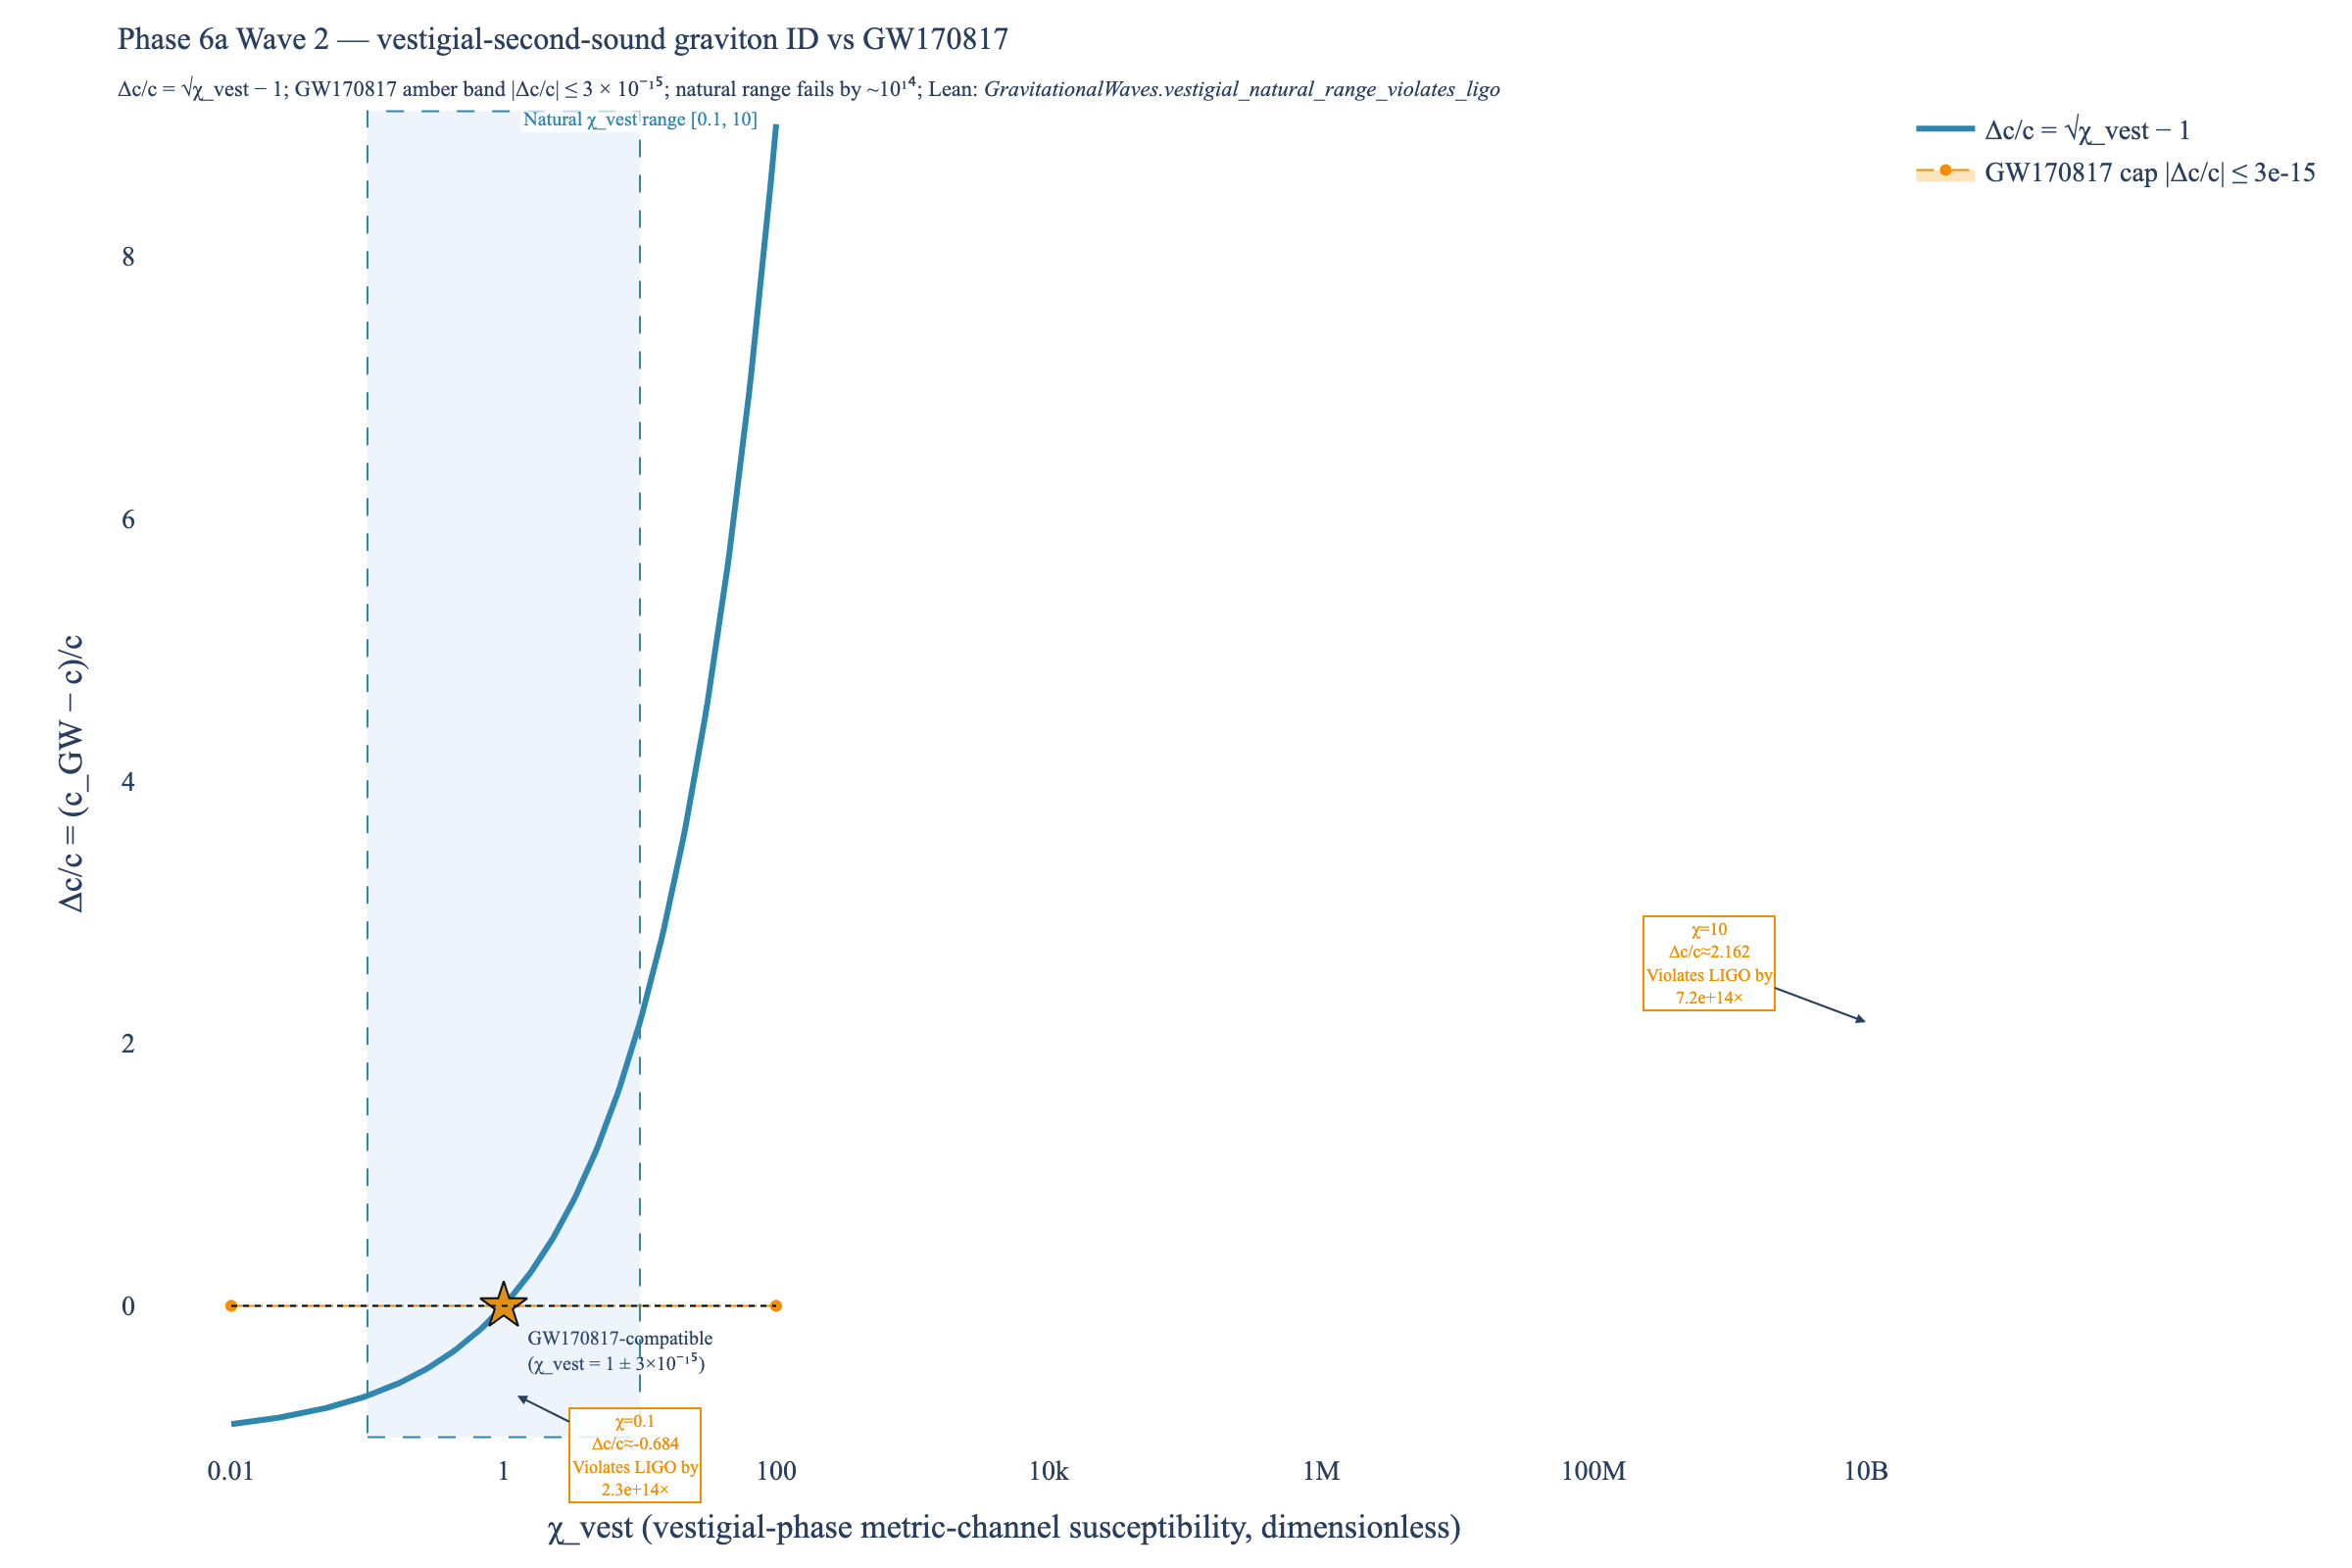
\includegraphics[width=0.96\columnwidth]{figures/fig_c_GW_vs_ligo_constraint.png}
  \caption{\textbf{Headline result.} The
  $\dccap = \sqrt{\chivest} - 1$ deviation across the natural
  $\chivest \in [0.1,10]$ range (pale blue band, dashed blue border)
  versus the GW170817~\cite{Abbott2017GW170817} multi-messenger cap
  $|\dccap| \leq 3\times 10^{-15}$ (amber, drawn at $\dccap = 0$ ---
  the cap's own width is far below one pixel at this scale). Over the
  natural range $\dccap$ sweeps $[-0.68, +2.16]$, exceeding the cap by
  $\sim 10^{14}\times$ \emph{at the endpoints} (orange callouts) and
  vanishing at $\chivest = 1$. The compatible $\chivest$ window
  $[(1-\tau)^2,(1+\tau)^2]$ is $10^{14}$ times narrower than the
  natural range and so renders as the single gold star --- note that it
  sits \emph{inside} the band, not beside it: the datum confines
  $\chivest$, it does not exclude the range. Lean witnesses:
  \texttt{ligo\_confines\_chi\_vest\_within\_natural\_range},
  \texttt{ligo\_window\_subset\_natural\_range},
  \texttt{vestigial\_natural\_range\_violates\_ligo}.}
  \label{fig:cGW}
\end{figure}

\paragraph{Tracked-hypothesis bundle.} Per the project's discipline
for non-derived identifications, we bundle the structural properties
of ``the vestigial mode is the graviton'' into a Lean Prop with
three independently load-bearing conjuncts:
\begin{equation*}
  \verb|H_VestigialModeIsGraviton|(\chivest)
  \equiv \chivest > 0
  \wedge \verb|LigoSatisfied|(\dccap(\chivest))
  \wedge |\dccap(\chivest)| < 1/2,
\end{equation*}
demanding positivity (P1), GW170817 compatibility (P2), and
sub-half-deviation $|\dccap| < 1/2$ as P3'. P3' is genuinely
independent of P1 (e.g.\ $\chivest = 1/10$ satisfies P1 with
$|\dccap| \approx 0.684 \not< 1/2$). The bundle is discharged at
$\chivest = 1$ (\texttt{H\_VestigialModeIsGraviton\_at\_one}) and
\emph{four} explicit falsifier theorems prove non-vacuity:
\verb|*_fails_at_natural_lower| (P2),
\verb|*_fails_at_natural_upper| (P2),
\verb|*_fails_at_zero| (P1), and
\verb|*_fails_at_quarter| (P3'; at $\chivest = 1/4$ the deviation is
exactly $\dccap = -1/2$, saturating the bound and isolating P3'
independence). The bundle's support over the natural-range prior has
measure $4\tau \approx 1.2\times 10^{-14}$ --- vanishingly small, but
non-empty, and containing $\chivest = 1$ --- and that is the
load-bearing falsifiability claim. (The
original Wave-2 P3 = $\forall c{>}0,\,\cGW(\chivest, c) > 0$ was
removed in the 2026-04-25 post-Wave-2 audit as redundant given P1;
P3' replaces it with a load-bearing quantitative constraint per the
project's preemptive-strengthening discipline.)

\paragraph{Phase~5y H1 caveat as a Lean endpoint theorem.} The
Phase 5y H1 deep research established that the Volovik identification
is not a \emph{derivation}: there is no first-principles bound fixing
the graviton-mode normalization in terms of the second-sound DOF.
We formalize this caveat as the endpoint theorem
\texttt{natural\_endpoints\_violate\_ligo\_window}: for $\chivest$
at either natural-range endpoint $\{0.1, 10\}$, no $c$-rescaling
gives a GW170817-compatible $\dccap$. The frame-independent form
\texttt{natural\_endpoints\_violate\_ligo\_for\_every\_c}
quantifies over all $c > 0$ explicitly, resting on
\texttt{c\_GW\_relative\_deviation\_eq}. Both concern the two
endpoints only; neither excludes interior values, and $\chivest = 1$
satisfies the cap (\texttt{ligo\_satisfied\_at\_chi\_one}).

%% ================================================================
\section{Discussion}
\label{sec:discussion}

\paragraph{What this rules out.} GW170817 does not exclude the
leading-order vestigial-second-sound identification outright: it
survives at $\chivest = 1$. What it rules out is the identification as
a \emph{generic} consequence of the natural range. Eq.~\eqref{eq:cGW}
requires $\chivest = 1 \pm 3\times 10^{-15}$, a fine-tuning so extreme
it cannot follow from a generic UV theory --- so any surviving version
of the identification owes an account of why $\chivest$ sits exactly
at unity.

\paragraph{What this does not rule out.} Three Phase~6 paths remain
open:
\begin{enumerate}
\item \textbf{Symmetry-driven $\chivest \to 1$ fixed point.} If a
deep-IR symmetry (e.g.\ Lorentz invariance of the emergent metric
sector) makes $\chivest = 1$ an exact fixed point of the RG flow, the
fine-tuning is structural rather than tuned. The present evidence
most favours this path: Volovik's own background returns $s_2 = c$
exactly, i.e.\ $\chivest = 1$, structurally. The value GW170817
selects is thus the value his construction already produces --- the
datum corroborates his result and indicts our substrate's failure to
reproduce it, not the identification. Phase~6 should examine
whether such a fixed point is realized in the ADW broken phase.
\item \textbf{Distinct metric-channel identification.} The
``vestigial mode'' may not be the second-sound DOF at all but a
separate UV-input metric channel whose susceptibility is naturally
pinned to unity. This was floated in~\cite{Volovik2022Counting} and
reads as the more likely interpretation under the Phase~5y H1
negative-evidence result. Phase~6e (full nonlinear emergent action)
is the natural venue for the disambiguation.
\item \textbf{Frequency-dependent $\chivest$.} Eq.~\eqref{eq:cGW} is
the leading term in a derivative expansion. If $\chivest$ varies
with frequency, the leading-order constraint could in principle be
relaxed by a near-cancellation in the LIGO band. The
SK--EFT dispersion correction is the leading frequency dependence in
the present framework, and this path is \emph{not} closed --- what we
can say is conditional.
\texttt{vestigial\_dispersion\_below\_ligo\_at\_inspiral\_peak}
takes $|\gamma| \leq 10^{-30}$ on $\Gamma_H/\cGW^2$ as a
\emph{hypothesis} and proves that under it the correction at the
$100\,\mathrm{Hz}$ inspiral peak stays inside the GW170817 tolerance.
It proves nothing about whether that bound holds: $10^{-30}$ is a
Phase~6a scaffold value, chosen so the correction would sit well below
the cap, and it is neither derived nor measured. So a
placeholder-sized correction would not relax the constraint; a larger
one is not excluded. The general form is
\texttt{dispersion\_within\_ligo\_iff}, a biconditional exchanging the
correction's tolerance for $|\gamma| \leq \mathrm{tol}/\omega$;
\texttt{dispersion\_correction\_abs\_bound},
\texttt{dispersion\_correction\_linear\_in\_gamma} and
\texttt{dispersion\_correction\_zero\_at\_no\_dissipation} fix its
magnitude, additivity and no-dissipation limit. A derivation of
$\Gamma_H$ from a microscopic matching is open.
\end{enumerate}

\paragraph{Comparison to the linearized-EFE wave.} The companion
linearized-EFE wave~\cite{Roehm2026LinearizedEFE} ships an
emergent-gravity identification \emph{compatible} with observation at
the natural-range level: the Sakharov--Adler form
$G_{\rm N,emerg} = \alpha_{\rm ADW} \cdot 12\pi/(N_f \Lambda_{\rm UV}^2)$
at $\Lambda_{\rm UV} = M_{\rm Pl}$ produces
$\alpha_{\rm ADW}^\star \in [0.40, 1.27]$ for SM $N_f$, sitting
inside the natural range $[0.1,10]$. The asymmetry between the two
waves is a feature of the program: the linearized-EFE
$G_{\rm N,emerg}$ depends on the Sakharov--Adler kernel computed at
the linearized level, where the relevant scale is $M_{\rm Pl}$;
$\cGW$ depends on the metric-channel susceptibility, where the
relevant scale is the dimensionless $\chivest$ which the natural
range happens to pin around 1 only by coincidence. GW170817 sees
the latter, and its bound is too tight to absorb the natural-range
spread.

\paragraph{Reproducibility.} The result is reproducible in two
layers. The Lean layer is \texttt{GravitationalWaves.lean} (32
theorems, zero \texttt{sorry}, zero new axioms, zero
\texttt{maxHeartbeats} overrides) at the project's pinned
Mathlib4 commit; the Python layer is \texttt{src/gravitational\_waves/}
with 49 \texttt{pytest} cases cross-checking every numeric quoted
in the abstract and figure caption. The headline figure
(\texttt{src/core/visualizations.py:fig\_c\_GW\_vs\_ligo\_constraint})
and its underlying numerics are committed-pinned.

%% ================================================================
\begin{thebibliography}{99}

\bibitem{Volovik2024Vestigial}
G.~E.~Volovik, ``Fermionic Quartet and Vestigial Gravity,''
JETP Lett.\ \textbf{119}, 330 (2024);
DOI: 10.1134/S002136402460006X.

\bibitem{Volovik2022Counting}
G.~E.~Volovik, ``Gravity from Symmetry Breaking Phase Transition,''
J.~Low Temp.\ Phys.\ \textbf{207}, 127 (2022);
DOI: 10.1007/s10909-022-02694-z.

\bibitem{Volovik2026SecondSound}
G.~E.~Volovik, ``Massless graviton in de Sitter as second sound,''
arXiv:2601.00639 (2026). \emph{The source of the
second-sound--graviton identification; derives $s_2 = c$ exactly and
leaves the graviton type open.}

\bibitem{Volovik2024VacuumDecay}
G.~E.~Volovik, ``From Landau two-fluid model to de Sitter Universe,''
arXiv:2410.04392 (2024).

\bibitem{Akama1978}
K.~Akama, Prog.\ Theor.\ Phys.\ \textbf{60}, 1900 (1978);
DOI: 10.1143/PTP.60.1900.

\bibitem{Diakonov2011}
D.~Diakonov, ``Towards lattice-regularized quantum gravity'',
arXiv:1109.0091 (2011).

\bibitem{VladimirovDiakonov2012}
A.~A.~Vladimirov and D.~Diakonov,
Phys.\ Rev.\ D \textbf{86}, 104019 (2012);
DOI: 10.1103/PhysRevD.86.104019.

\bibitem{HebeckerWetterich2003}
A.~Hebecker and C.~Wetterich,
Phys.\ Lett.\ B \textbf{574}, 269 (2003);
DOI: 10.1016/j.physletb.2003.09.010.

\bibitem{Wetterich2022}
C.~Wetterich, JHEP \textbf{06}, 069 (2022);
DOI: 10.1007/JHEP06(2022)069.

\bibitem{Vergeles2025}
S.~N.~Vergeles, Phys.\ Rev.\ D \textbf{112}, 054509 (2025);
DOI: 10.1103/PhysRevD.112.054509.

\bibitem{Abbott2017GW170817}
B.~P.~Abbott \emph{et al.}\ (LIGO/Virgo, Fermi GBM, INTEGRAL),
Astrophys.\ J.\ Lett.\ \textbf{848}, L13 (2017);
DOI: 10.3847/2041-8213/aa920c.

\bibitem{BakerBellini2017}
T.~Baker, E.~Bellini, P.~G.~Ferreira, M.~Lagos, J.~Noller and I.~Sawicki,
Phys.\ Rev.\ Lett.\ \textbf{119}, 251301 (2017);
DOI: 10.1103/PhysRevLett.119.251301.

\bibitem{CreminelliVernizzi2017}
P.~Creminelli and F.~Vernizzi,
Phys.\ Rev.\ Lett.\ \textbf{119}, 251302 (2017);
DOI: 10.1103/PhysRevLett.119.251302.

\bibitem{SaksteinJain2017}
J.~Sakstein and B.~Jain,
Phys.\ Rev.\ Lett.\ \textbf{119}, 251303 (2017);
DOI: 10.1103/PhysRevLett.119.251303.

\bibitem{EzquiagaZumalacarregui2017}
J.~M.~Ezquiaga and M.~Zumalac\'arregui,
Phys.\ Rev.\ Lett.\ \textbf{119}, 251304 (2017);
DOI: 10.1103/PhysRevLett.119.251304.

\bibitem{Roehm2026LinearizedEFE}
J.~G.~Roehm, ``Linearized Einstein Equations from
Anderson--Higgs Tetrad Condensation'',
\emph{SK--EFT-Hawking project, in preparation}, 2026
(\texttt{papers/paper23\_linearized\_efe/}).

\end{thebibliography}


%% ─── Lifted from _phase6o_W1b_lean_only (§4) — 2026-05-06T15:42:03Z ───
%% \section{G4 Kerr-Schild double-copy on Petrov-D analog gravity}
%% \label{sec:l1-_phase6o_W1b_lean_only}

%% Insertion point hint from PAPER_DRAFT_MAPPING.md: §4
%% Lift notes: D.2 absorption: Phase 6o W1b Kerr-Schild single-copy as alternative substrate context to vestigial graviton; cross-ref-only
%% NOTE: absorption DECLINED 2026-05-06; see papers/L1/append_log.json. The
%% three work markers formerly here were vestigial bookkeeping from that
%% abandoned lift, not outstanding work on L1, and were removed 2026-08-14
%% (review:2026-08-14-l1-stage13:L1:7.1). Had the lift proceeded it would
%% have owed: content from papers/_phase6o_W1b_lean_only/paper_draft.tex,
%% numerical claims traced via formulas.py / counts.tex, and primary-source
%% cache entries for its citations.

%% (Section heading + label commented out 2026-05-06 Session 2: empty post-bibliography stub from bundle_append.py default-insertion; bookkeeping anchor preserved as LaTeX comment, no rendered content. Append-log entry retains source-contribution registration.)
%% ─── End lift from _phase6o_W1b_lean_only ───

\end{document}
